\documentclass{article}
\usepackage[utf8]{inputenc}
\def\MakeUppercaseUnsupportedInPdfStrings{\scshape}
\usepackage{hyperref}
\usepackage{graphicx}

\title{Aubo Guides and Training material}
\author{Lead Robotics}
\date{May 2022 v0.1.0}

\begin{document}

\maketitle

\tableofcontents

\section{This document} 
This document is meant to supplement the aubo manual. The manual can be found at the \href{https://github.com/MalteNJLead/LeadPublic/tree/main/Aubo}{Aubo website} or at the \href{https://github.com/MalteNJLead/LeadPublic/tree/main/Aubo}{Lead Robotics public repository}.

Where the manual describes every button and feature in the robot. This manual aims to give a more thorough and step by step walkthrough of how to implement features in your programs and robot setups.
  
It is split into two basic sections. The fundamentals section is for basic usage and getting started with a first program. The advanced usage section covers everything else in no particular order. Consult the table of contents if you are looking for a particular feature. 

\section{Fundamentals}
This  section is for fundamental use of the robot. Anybody who operates the robot is encouraged to study this section. 

\subsection{Startup}
\label{subsec:Startup}
Another description of the startup procedure can be found in the Aubo manual in the section 'Getting Started'.

TLDR: Plug everything in. Turn the large switch on the controlbox. Wait until the standby light starts. Then hold the power button on the teachpendant for around 2 seconds. 

After startup the Aubo programming environment (AuboPE) will start automatically. Login with the default password: '1' and press save, and then startup on the popup. The manipulator arm should now power on, the brakes will click, and the AuboPE UI should appear.  

For another 
\begin{itemize}
  \item Connect the three cables to the controlbox. Connect the other ends to the manipulater arm, 230VAC power and the teacpendant screen respectively.
  \item Turn the box on. On the compact box the switch is located right above the power cord plugin. On the large box the breaker is round and jutting out of the front of the box. After turning the switch you should hear the fans start in the box.
\begin{center}
  \makebox[\textwidth]{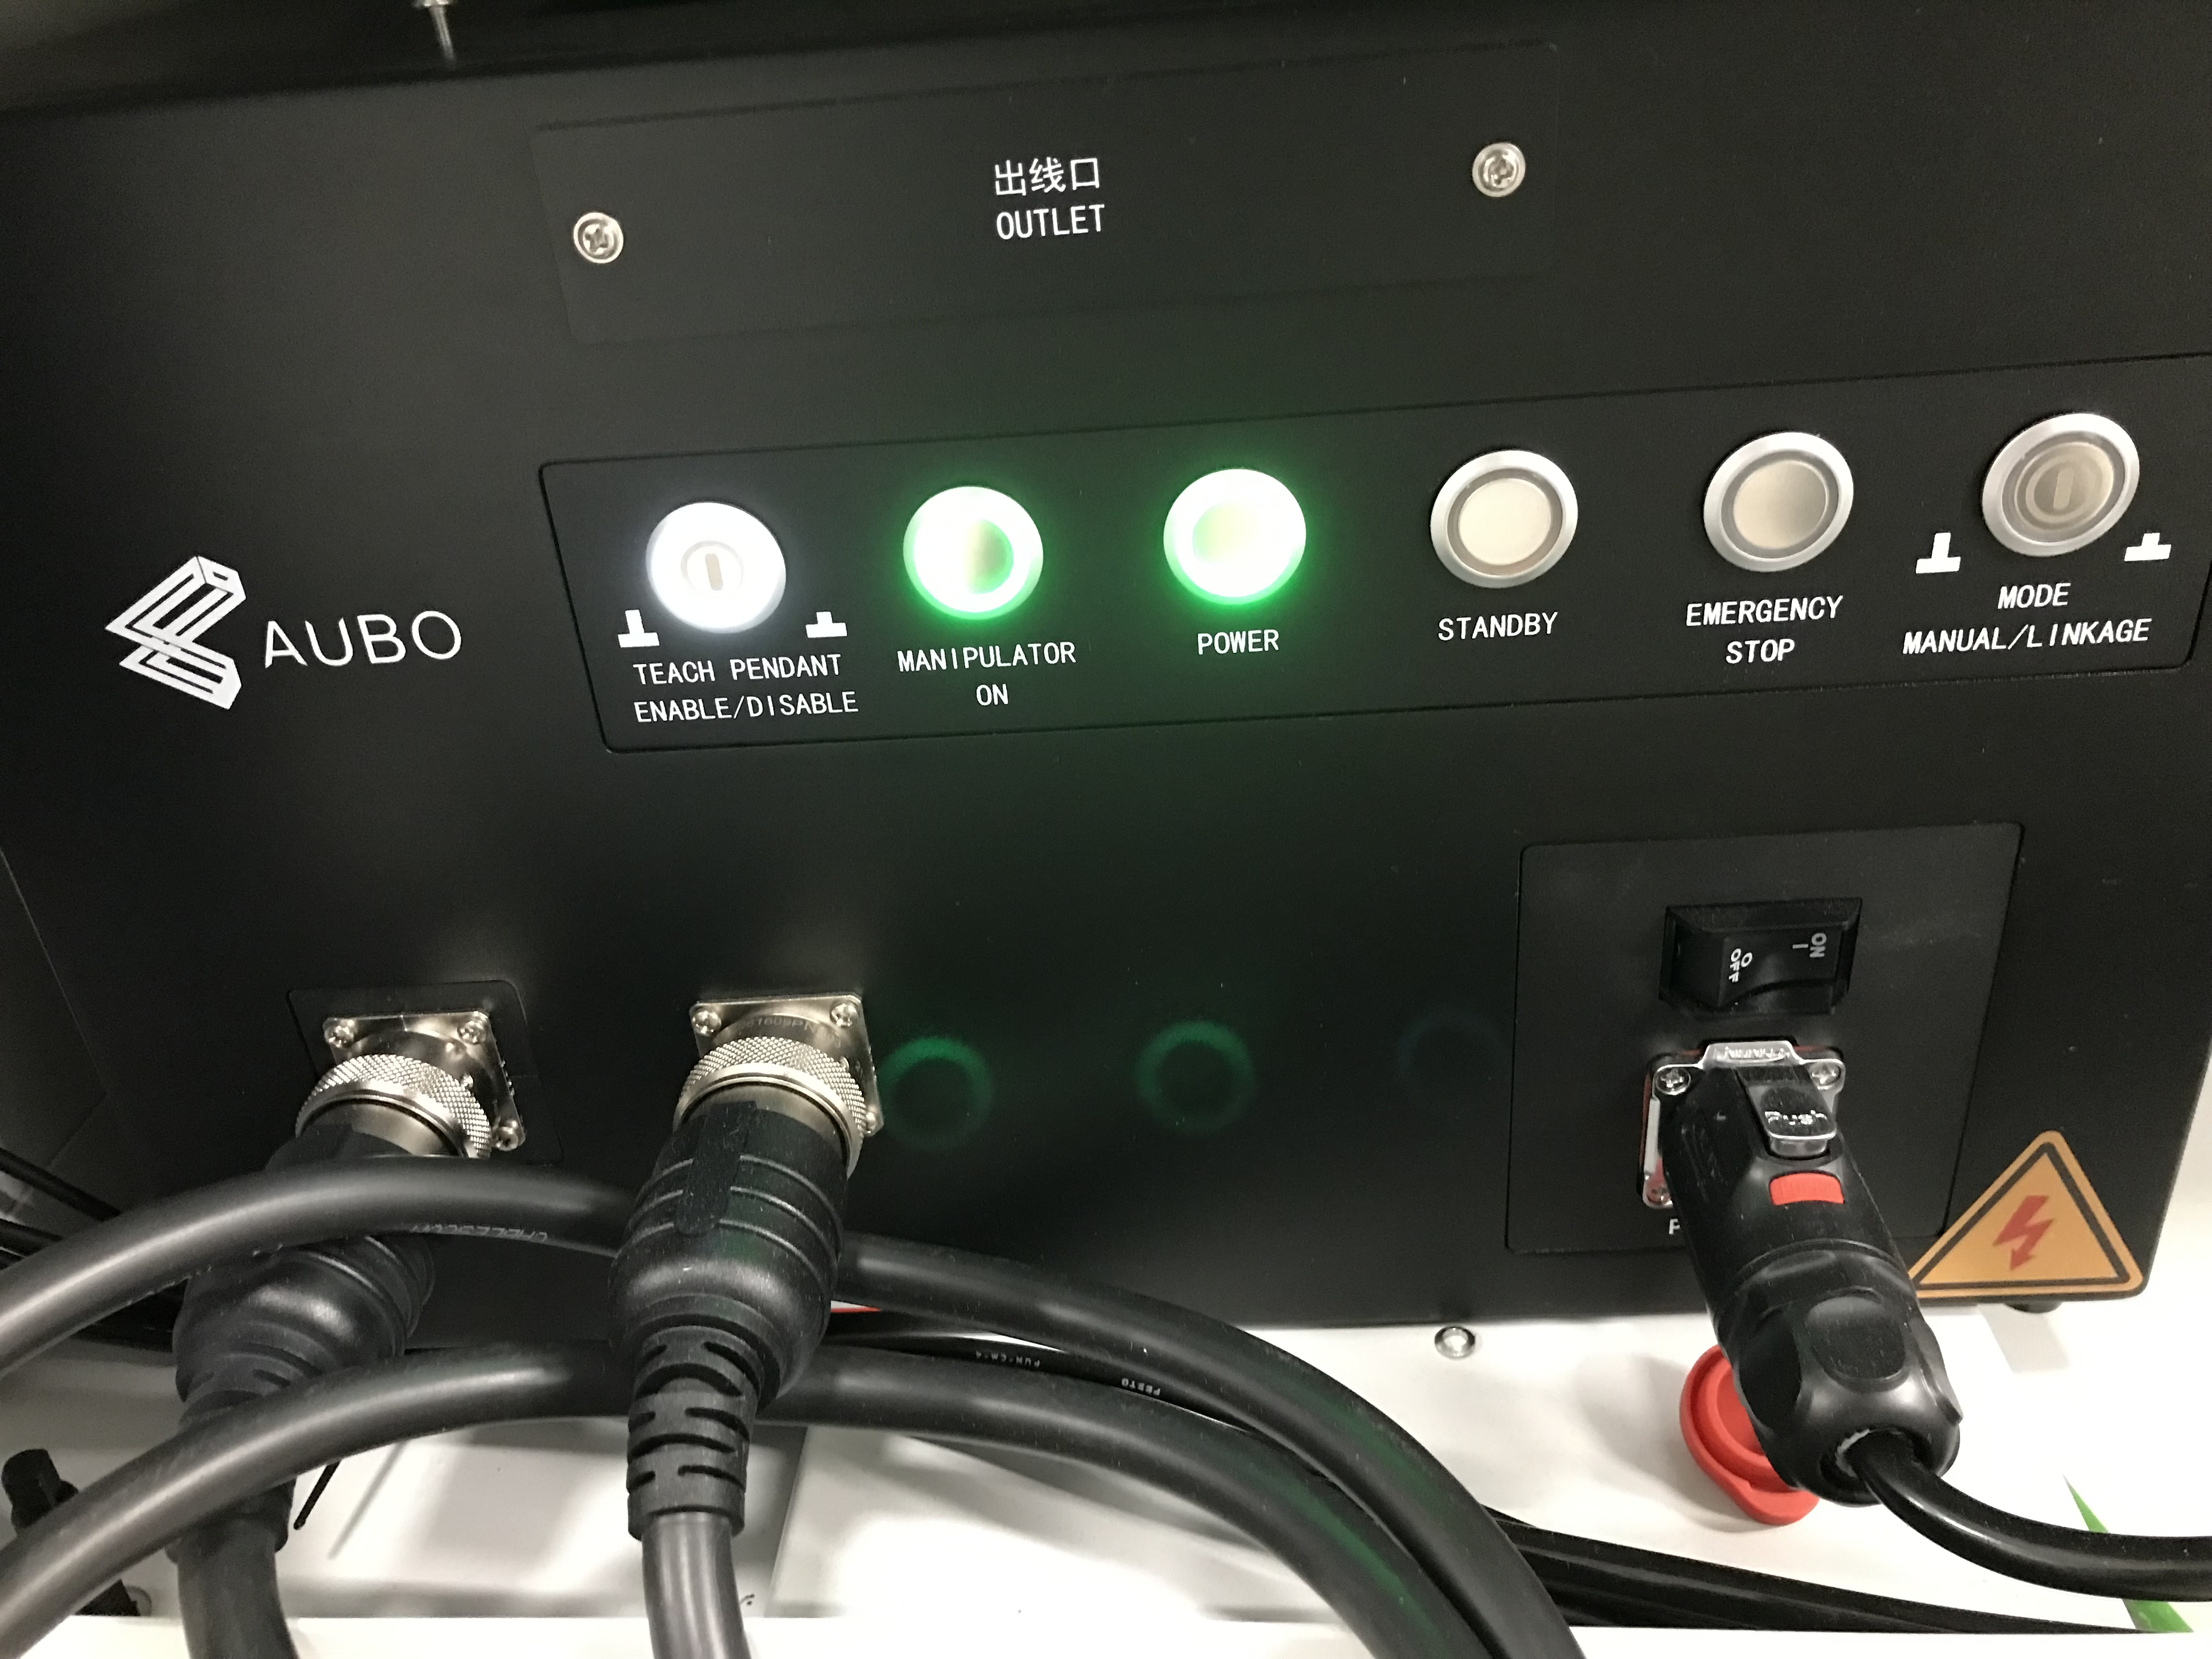
\includegraphics[width=\textwidth]{../../Images/FrontCompactAuboBox.jpg}}
\end{center}
\item Wait for the ‘Standby’ light to turn on with a solid orange light. 
\item If the Emergency stop light is lit up in red make sure to clear the emergency stop buttons. There is one on the teachpendant and one on the large control box. 
\item Now get the teachpendant and press and hold the power button in the top-left corner for at least 1s. The button should light up blue.
\item Wait for the teachpendant to start. 
\item A guarantee disclaimer might appear, click agree to continue. 
\item You should now see a login screen and a desktop. 
\item Close the login screen for now, we will get to the robot program later. 
\item You should now only see the desktop with 3 shortcuts -> ‘AUBOPE’, ‘Files’ and ‘Terminal’. AUBOPE is the robot software. This will re-open the login screen and get us into the robot programming. Files opens the filesystem. Terminal opens a bash terminal.
\end{itemize}

\subsection{Shutdown} 
Press and hold the power button on the topleft of the teachpendant for at least a second.

The Screen should go black. 

The Robot is ready to start back up when the ‘standby’ light on the control box lights up orange. 

\subsection{Logging in}
\label{subsec:login}
After restart the login screen should appear automatically. Otherwise doubleclick on the AUBOPE shortcut on the desktop. Type the password, default is '1' and press login. 

The next screen is called 'Robot Init Form', press save and then startup to proceed. The robot will now go through an initializing. You should hear the brakes click.

The teachpendant should then show the robot software user interface.  


\subsection{Moving the Robot}
You can move the robot in two ways. 
You can press the black button on the right side of the teachpendant. The button is a three position switch, where the middle position will release the brakes and let you drag the robot around.

The second method uses the teachpendant. Go to the leftmost menu 'RobotTeaching'. Here you can move the robot in various ways.

Task1: Try both ways of moving the robot. 
Task2: Try moving with regards to position and orientation. 
Task3: Move joints directly
Task4: Try moving in stepmode. 
Task5: There is an area direcly above and below the base of the robot, that the flange cannot enter. Try moving the robot into this singularity. 
  
\subsection{UI Programming} 

The programming menu in AuboPE lets you construct lua programs from the UI. In this menu you can save and load projects and edit them with new instructions. Instructions include basic proramming blocks like if statements and loops and also movement commands and threads. 
When you have built and saved a program you can have the robot execute it by clicking start in the bottom left corner. For the project to start the robot needs to be moved to the first movement position in the program. To do this hold down the red Auto button. 

task1: Create a project that moves the arm between two points in a loop and execute it. 

\subsection{User I/O}

\section{Advanced Use}
\subsection{Programming in Lua}
\subsection{User Coordinate Systems}
\subsection{Security Features}

\subsubsection{Emergency stop}
Emergency stop is on SI00 og SI10. Anything other than a continuous high signal on these inputs and the robot will enter emergency stop. 

S00 and S10 will output a high signal if the robot is in an emergency state, but will be nominally low. 



\subsection{Modbus Communication}
\subsection{Linkage Mode}
\subsection{Tool I/O}
\subsection{Sharing Internet}
If there is no cable connection to supply the AUBO robot with internet you can connect it through a PC with a wifi connection. 

For windows 10: 
First step connect the ethernet cable.
Next we have to define static matching IP's for both the robot and the PC. 
On windows you go to 
Then define a static ip for both robot and the pc's ethernet connection. 
In windows that would be
\begin{itemize}
\item Open controlcenter
\item Click network and internet
\item Click network and sharing center
\item Select the ethernet connection under active networks 
\item Open properties
\item define a new static Adressing. fx. IP: 192.168.137.4, with subnetmask 255.255.255.0 and leave the standard gateway blank. For DNS you could use 8.8.8.8 with alternative 8.8.4.4.
\end{itemize}

On the robot changing the static IP is done with the file /etc/network/interfaces or through system settings. 
write out the ethernet specifications. An example could be. 
\#eth3
auto eth3 
iface eth3 inet static 
address 192.168.137.2 \#static Ip of robot
gateway 192.168.137.1 \# since we are routing internet through the PC we use its IP as the gateway. 
netmask 255.0.0.0  
\#eth3 config finished

make sure to save the changes and the perform a reboot for them to take affect. 
Now you should have a connection between laptop and robot, which can be tested by pinging the opposition from either device. Fx in the robot terminal write \$ping 192.168.137.1.
 
The last step is to allow sharing of internet in windows. Go again to controlcenter -> network and internet -> network and sharing center here select your active wifi connection (that gives you access to the internet). go to properties -> sharing and allow sharing over the ethernet connection (or whatever your cabled connection is called)

Now you should be able to access the internet on the robot. Test it by visiting a webpage or pinging google at 8.8.8.8 or pinging something else. 

\subsection{Remote Access}
\subsection{Updating}
\subsection{Virtual machine}
\label{sec:virtual}

1.	Install virtual machine environment
Find and install a virtual machine. I use vmware: https://www.vmware.com/products/workstation-player/workstation-player-evaluation.html

2.	Open Aubo Virtual machine
The VM can be found on aubo’s homepage. But this is a direct link to the drive where they host it:  https://drive.google.com/drive/folders/1vxmE4JyKkqD4IaGncI1EtJIXRtCnlECY 
Make sure you get the all the parts and unzip them. Now you should have a folder called $$'Aubo-ORPE_V4.0.x_Release'$$ . This folder contains the virtual machine. 
Open the virtual machine on your environment of choice. 
On VMware you press open VM and navigate to $$Aubo-ORPE_V4.0.x_Release/ aubo.vmx\setminus$$ . Then the machine will be listed under the name aubo. Right click on the name to access the settings in order to change the name and maybe adjust the allocated RAM for the VM. Then click ok and press “play virtual machine”.  A popup will appear, mark of that you copied the VM. And then Ubuntu should start. 

3.	Update Aubo virtual machine
Update Aubo to the newest version. See https://drive.google.com/drive/folders/1e2sAyCd5S1s4jH7FRyMwZzTy7VTZb2NE for details. 
Remember the default password is: 1 
Also if the resolution is small, moving the virtual machine window about seems to fix it (on vmware). 
Also you might want to change the keyboard layout. 
To move files into VMWare you can use an external harddrive or you can setup a shared folder between host and VM.

\subsection{Plugin Design}

The recommended way to build plugins is to do it within the virtual machine. See section \ref{sec:virtual}. 
After opening the VM locate project and build it.
Now the desktop toolbar disappears in the new update but you can get it back by typing this command in the terminal: 
\$ unity\& 
Now go to the top left corner and search for QTcreator community edition. 
When you open QT the plugin example should be in the recent project list. Otherwise the path is: $$/root/Workspace/PluginTest/ORPE_Extention_SDK.pro$$
Open the project and build it. 
This creates the plugin file(s) (with  the .so file ending) under: $/root/Workspace/build-ORPE_Extention_SDK-qt5_{5_1}-Debug/*$

Using the plugins.
Moving these .so plugin files into the robot filesystem under: $$/root/AuboRobotWorkSpace/teachpendant/lib/teachpendant/$$
And performing a reboot of the robot or virtual machine should have your new tabs show up within AuboPE. The example creates a tab under extensions -> peripherals -> Robotiq2F.


\subsection{Palletizing Software}

\subsection{opening system settings}
\label{subsec:OpenSystemSettings}
The robot runs on ubuntu 14.04, and there are a number of reasons you might want to access the ubuntu settings. Fx setting up IP's and changing keyboard layout. 

\begin{itemize}
	\item Startup the robot and close the login screen so you are looking at the desktop
	\item Open a terminal, by double tapping the icon. (or plug in a mouse and doubleclick on it)
	\item Enter command:$'unity\&’$, beware if you haven't changed the keyboard layout the $‘\&’$ sign will be located on $'shift+7’$ as on a US keyboard not on $‘shift+6’$ as with a Danish keyboard. This command will start the unity desktop environment and give you a toolbar on the left side of the screen.
	\item Open system settings either on the toolbar to the left or with the dropdown menu in the topright corner of the screen. The icon is a gear and a wrench. 
\end{itemize}

\subsection{Changing Keyboard Layout}
The keyboard layout will normally be set to English(US). This might be fine but be aware, if you are using a different keyboard, that some keys might be placed differently. If you want to change the layout continue in this section.

\begin{itemize}
\item startup and open system settings. See sections \ref{subsec:Startup} and \ref{subsec:OpenSystemSettings}
\begin{center}
  \makebox[\textwidth]{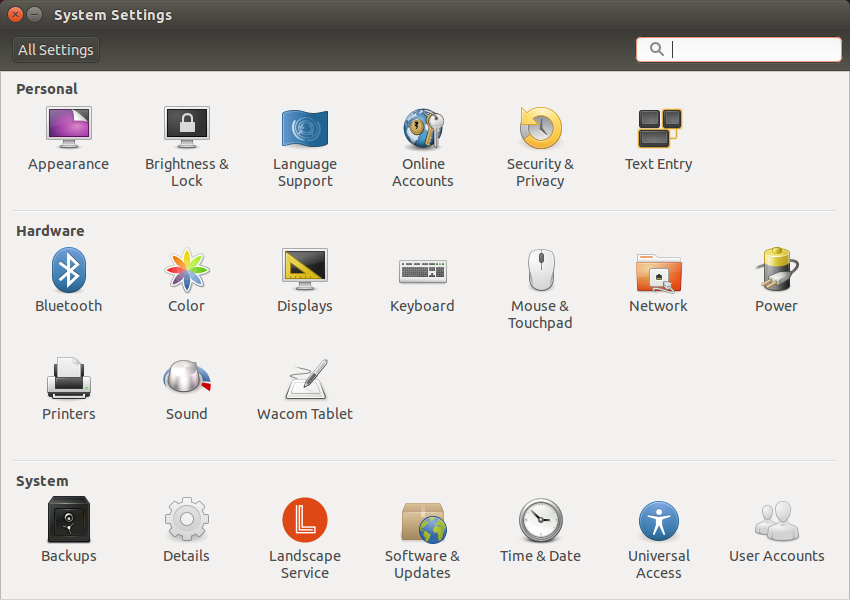
\includegraphics[width=\textwidth]{../../Images/systemSettings.png}}
\end{center}
\item In system settings open $‘Text Entry’$
\begin{center}
  \makebox[\textwidth]{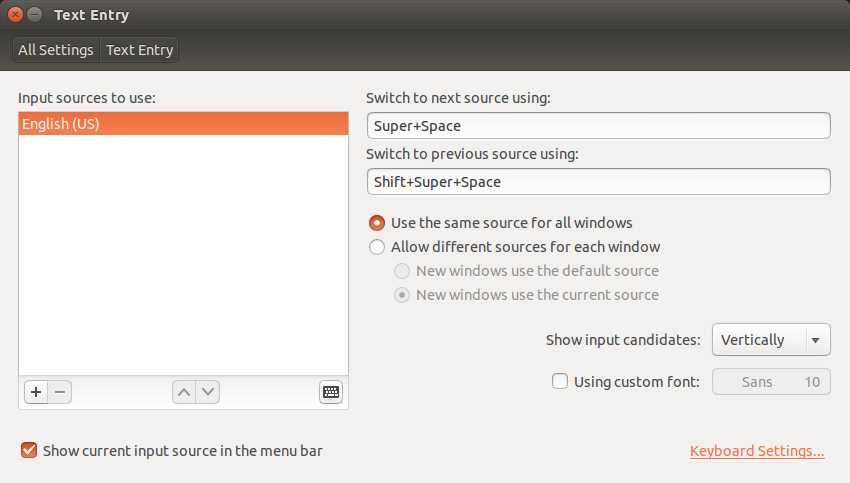
\includegraphics[width=\textwidth]{../../Images/TextEntry.png}}
\end{center}
\item Under the list of input sources on the left press the ‘+’ button to add an input source. 
\item Find your desired layout in the list (fx. Danish). 
\begin{center}
  \makebox[\textwidth]{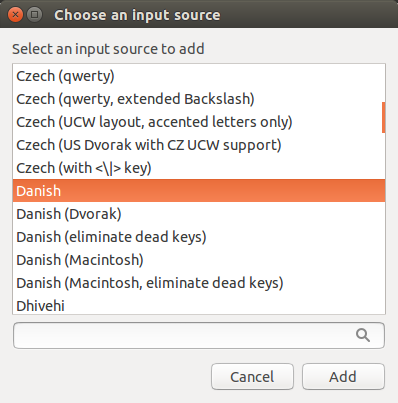
\includegraphics[width=\textwidth]{../../Images/addingDanishLayout.png}}
\end{center}
\item Select your layout and press add. 
\item The name of your layout should now appear in the list of input sources marked with orange.
\begin{center}
  \makebox[\textwidth]{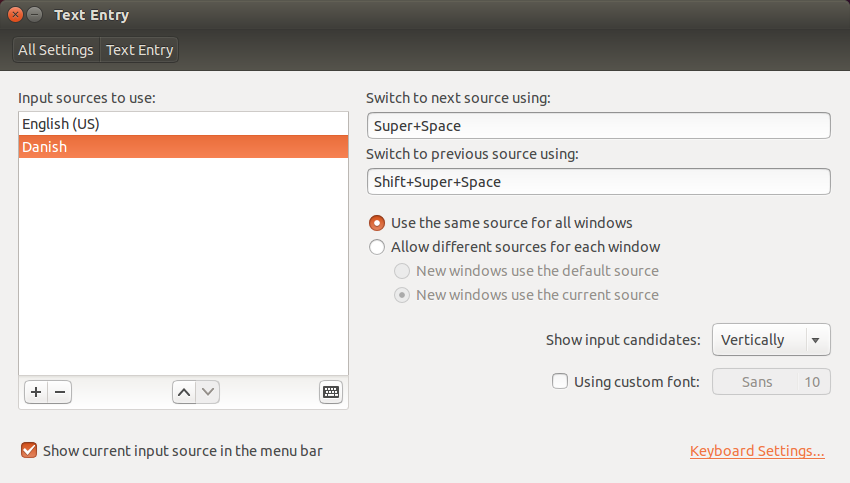
\includegraphics[width=\textwidth]{../../Images/danishAddedToInputSources.png}}
\end{center}
\item Close the Text Entry box.
\item Go to the top right corner of the screen and click where it says ‘En’ for English. This will open a dropdown menu where you can now select your newly added keyboard layout.
\begin{center}
  \makebox[\textwidth]{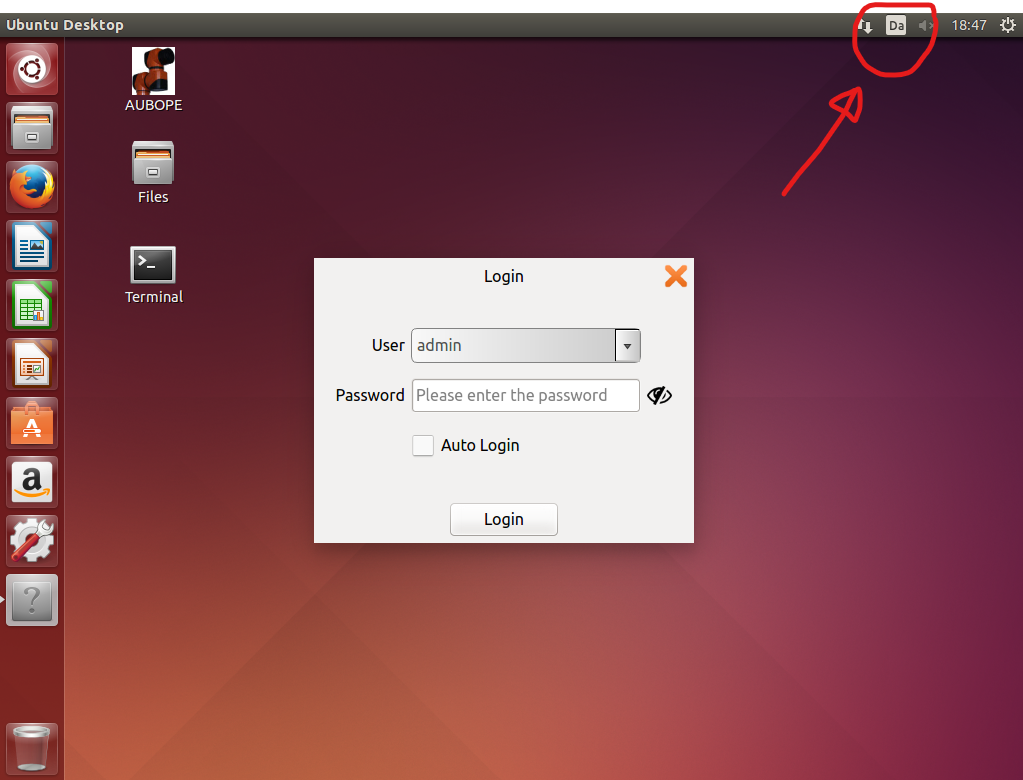
\includegraphics[width=\textwidth]{../../Images/LanguageChange.png}}
\end{center} 
\item You should now have a different keyboard configuration. Test it by opening a terminal and typing some symbols.
\end{itemize}

\subsection{Set static IP}
There are two main ways to change the static IP. 

You can write changes directly in the file /etc/network/interfaces or you can do it through system settings. 

I recommend doing it through system settings. 

\subsubsection{Using System Settings}
\begin{itemize}
\item Start robot and open system settings (see \ref{subsec:Startup} and \ref{subsec:OpenSystemSettings})
\begin{center}
  \makebox[\textwidth]{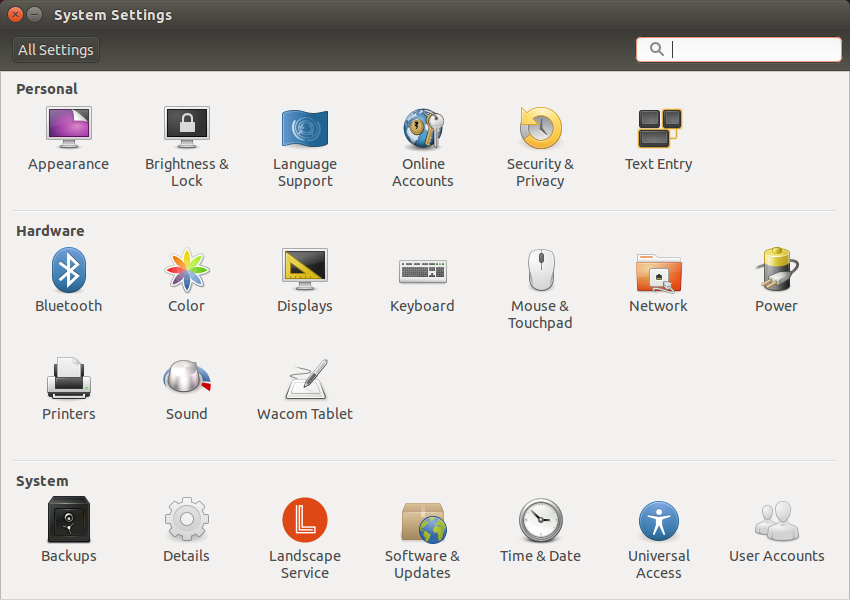
\includegraphics[width=\textwidth]{../../Images/systemSettings.png}}
\end{center}
\item Doubleclick on network

\begin{center}
  \makebox[\textwidth]{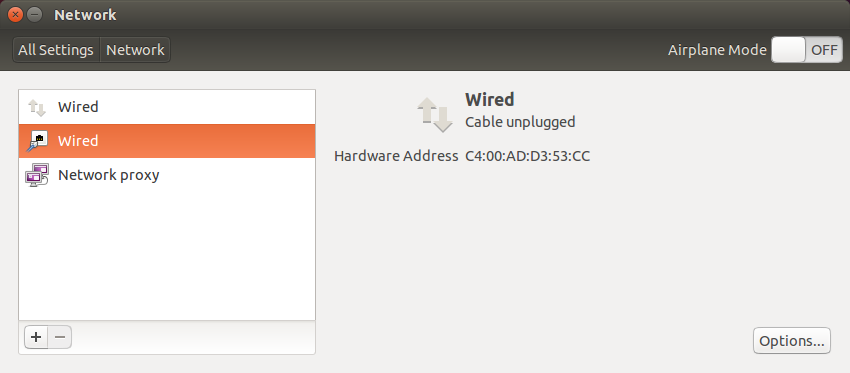
\includegraphics[width=\textwidth]{../../Images/networkWired.png}}
\end{center}
\item Select wired. The icon with the ethernet port not the arrows.
\item click options
\begin{center}
  \makebox[\textwidth]{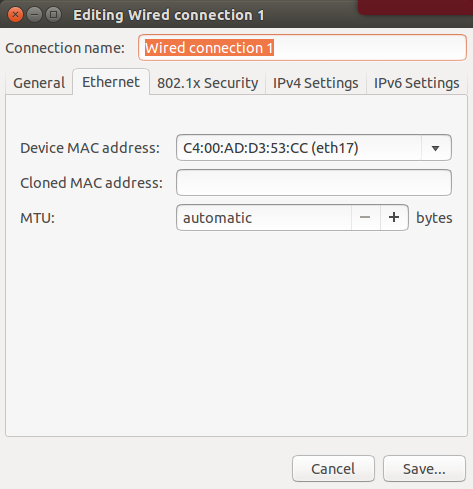
\includegraphics[width=\textwidth]{../../Images/wireOptionsEthernet.png}}
\end{center}
\item Select the IPv4 settings tab
\begin{center}
  \makebox[\textwidth]{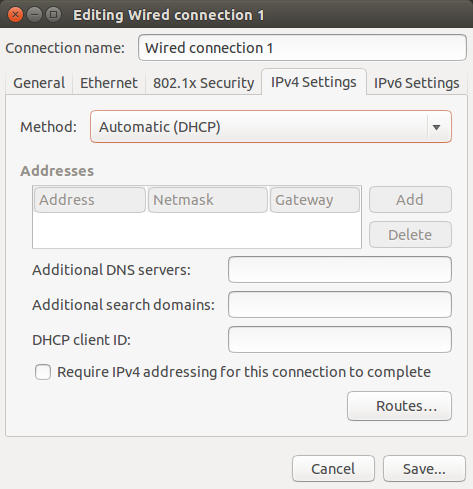
\includegraphics[width=\textwidth]{../../Images/IPv4SettingsAutomatic.png}}
\end{center}
\item In the Method dropdown bar select $'manual'$ 
\begin{center}
  \makebox[\textwidth]{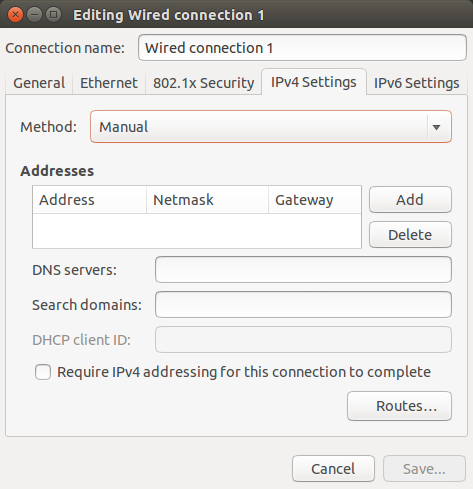
\includegraphics[width=\textwidth]{../../Images/ipv4SettingsManual.png}}
\end{center}
\item Click add and type in your desired IP, mask and gateway. 
\begin{center}
  \makebox[\textwidth]{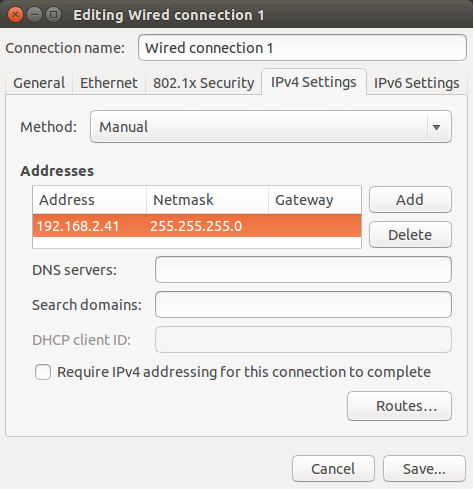
\includegraphics[width=\textwidth]{../../Images/IPv4SettingsWithAdress.png}}
\end{center}
\item Click save. 
\end{itemize}
The robot should now have a static IP. You can test it by connecting a computer and pinging the robot on its new adress. 

\subsubsection{Using interfaces file}
Open a terminal and type the command $ifconfig$. 
This will list your connection. Find the name of your ethernet connection fx. $'eth3'$ and write out the ethernet specifications. An example could be. 
\#eth3
auto eth3 
iface eth3 inet static 
address 192.168.137.2 \#static Ip of robot
gateway 192.168.137.1 
netmask 255.255.255.0  
\#eth3 config finished
navigate to /etc/network/interfaces, and open it with a text editor. 
add your specification at the bottom of the file.
Now either restart the network config, or the entire system.

\subsection{update}
Check out the guides \href{https://drive.google.com/drive/folders/1e2sAyCd5S1s4jH7FRyMwZzTy7VTZb2NE}{here}. For more info. 

\subsubsection{Update via USB}
\begin{itemize}
\item Acquire USB with update software. the software is a compressed file ending in .aubo. 
\item Plugin the usb. 
\item Startup and login to the aubo robot. See \ref{subsec:Startup} and \ref{subsec:login} 
\item Click on the settings tab at the top. 
\begin{center}
  \makebox[\textwidth]{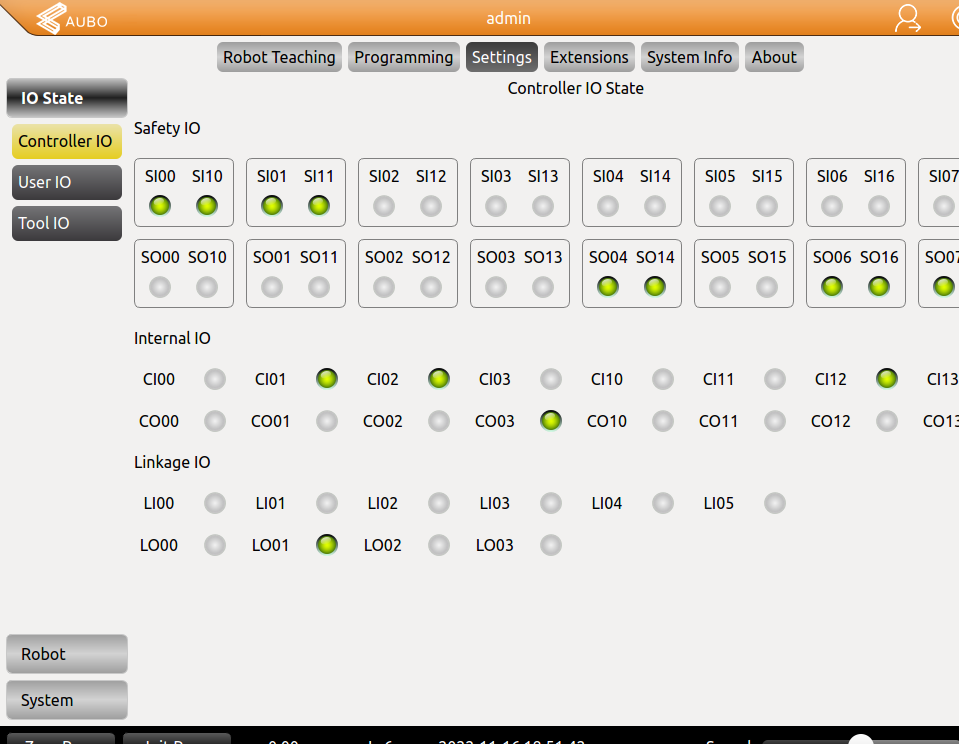
\includegraphics[width=\textwidth]{../../Images/settings.png}}
\end{center}
\item select $'system'$ in the bottom left. 
\begin{center}
  \makebox[\textwidth]{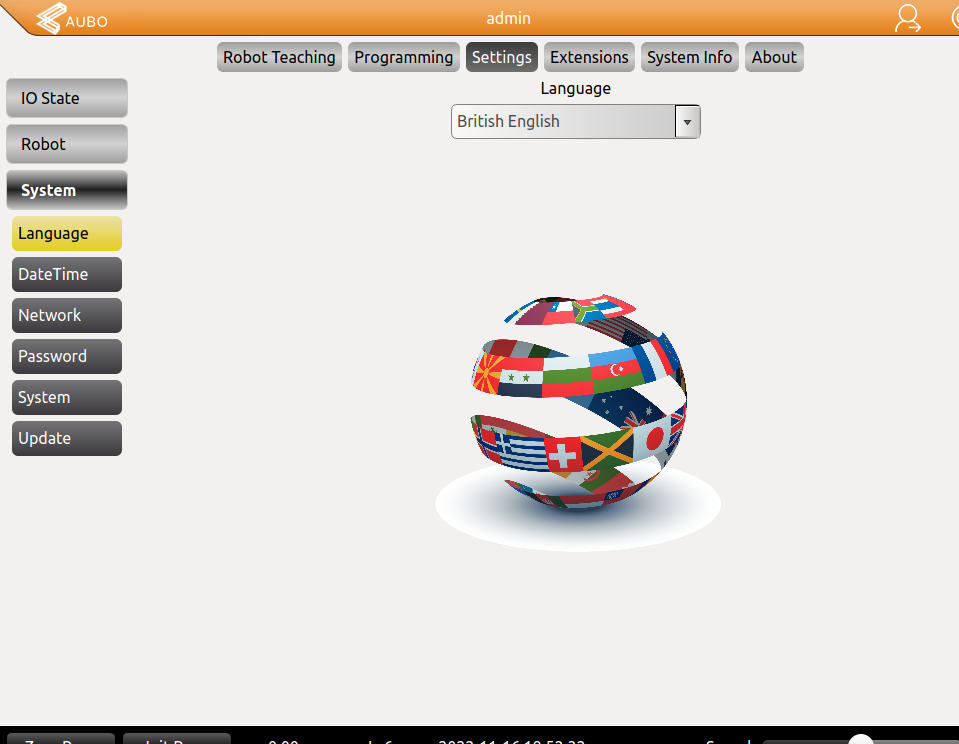
\includegraphics[width=\textwidth]{../../Images/settingsSystem.png}}
\end{center}
\item Select update on the left. 
\begin{center}
  \makebox[\textwidth]{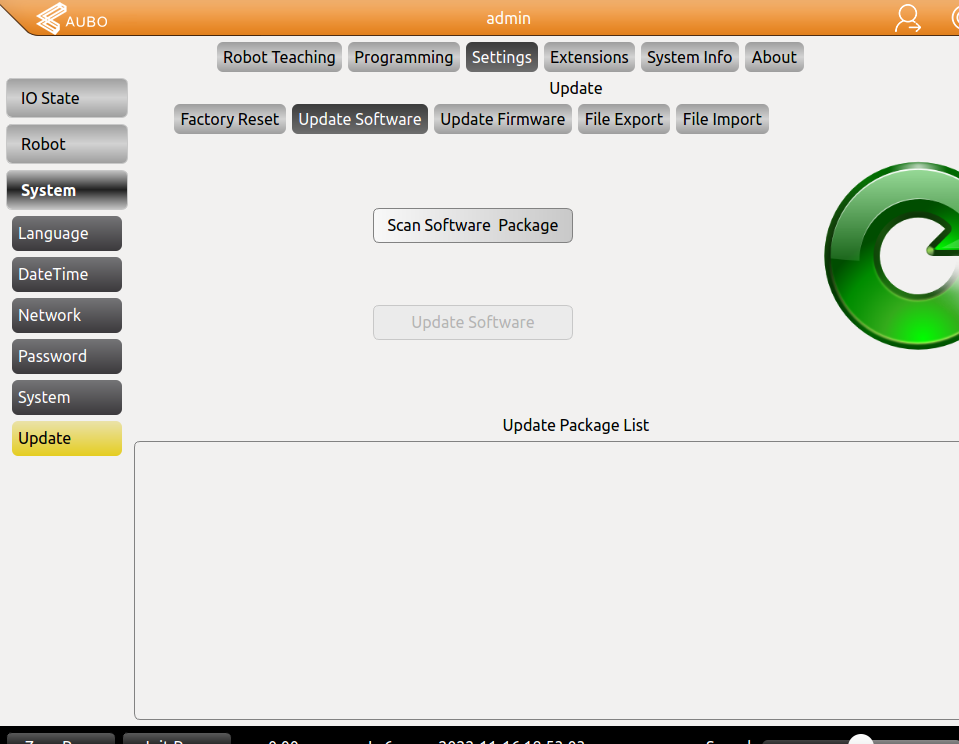
\includegraphics[width=\textwidth]{../../Images/update.png}}
\end{center}
\item Click on the $'Scan Software Package'$ button in the center of the screen. the names of the update files on your USB should appear in the list.
\begin{center}
  \makebox[\textwidth]{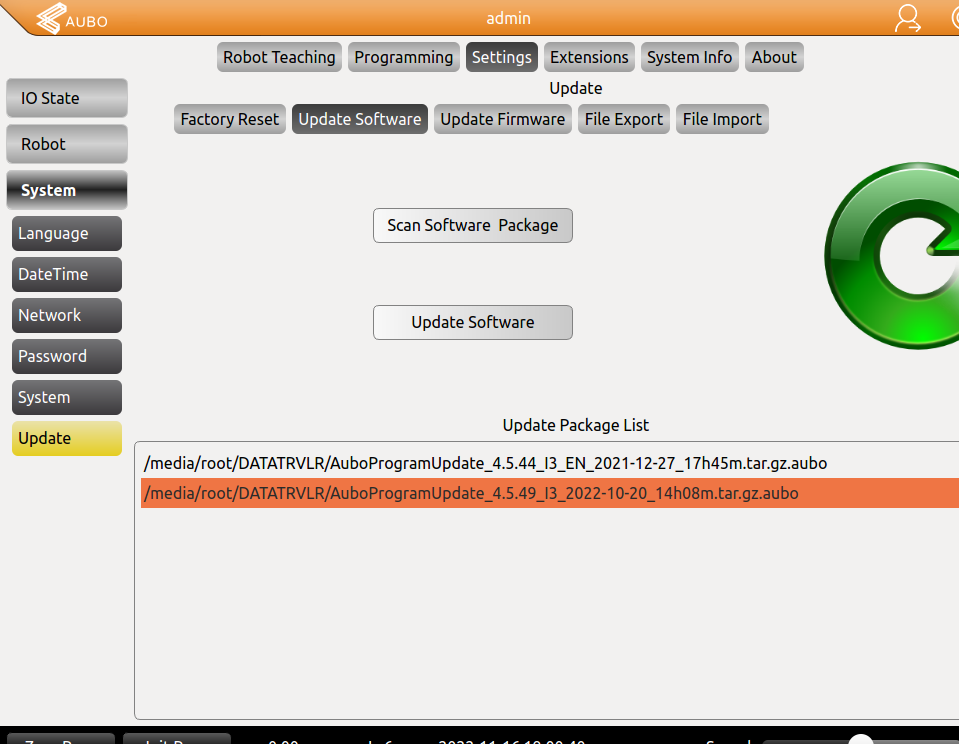
\includegraphics[width=\textwidth]{../../Images/lisrofUpdateFiles.png}}
\end{center}
\item Select your desired update file and press $'Update Software'$
\item A confirmation window will appear. Press $'yes'$ you do want to update.
\item Wait for the update to finish. This will take about 30 seconds. 
\item The program will tell you to restart. Click $'ok'$, and then $'yes'$ to shutdown.
\item Start the robot back up
\item The robot might have switched language. Dont panic. The program is still the same the text is just different. 
\item login. 
\item if the language is different go to settings and then to system. Use the previous screenshots in the guide to locate the buttons. The screen shows a sphere made of flags. Use the dropdown menu to change languages.
\item Go to the about tab and in the top right
\item Check that the Teachpendant Version has been updated. 
\end{itemize}

\subsection{Using Backups} 
With backups you can transfer all programs, variables and settings onto a new system. 

\subsubsection{Creating a Backup}
\begin{itemize}
\item plugin a usb. 
\item Startup and login to the aubo robot. See \ref{subsec:Startup} and \ref{subsec:login}
\item Go to the $'Settings'$ tab.
\begin{center}
  \makebox[\textwidth]{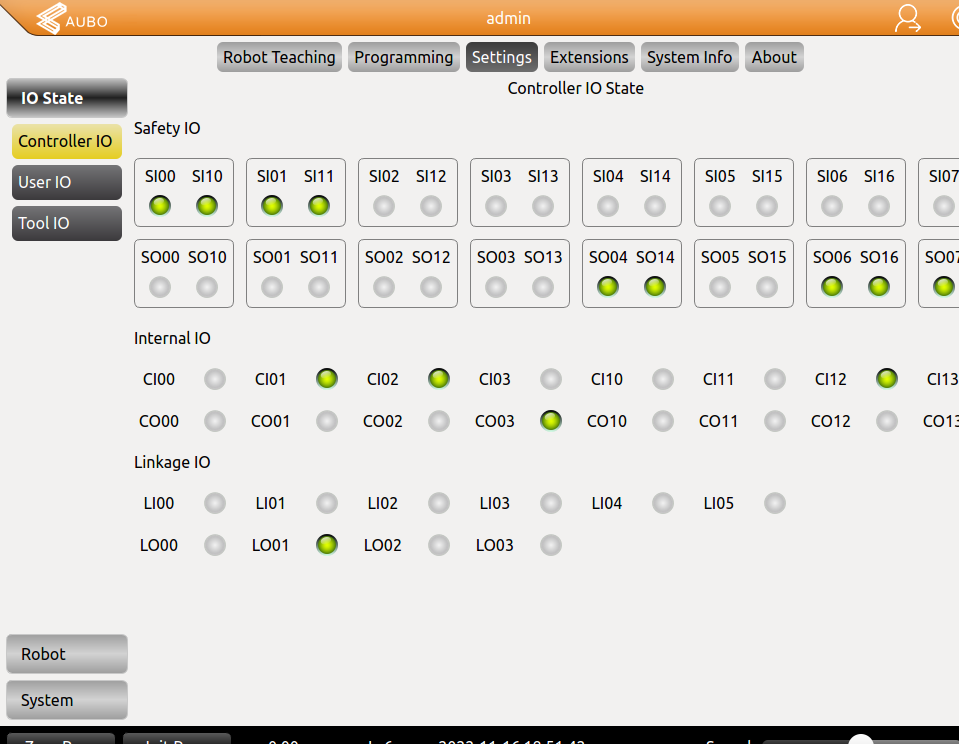
\includegraphics[width=\textwidth]{../../Images/settings.png}}
\end{center}
\item open the $'System'$ tab on the left
\begin{center}
  \makebox[\textwidth]{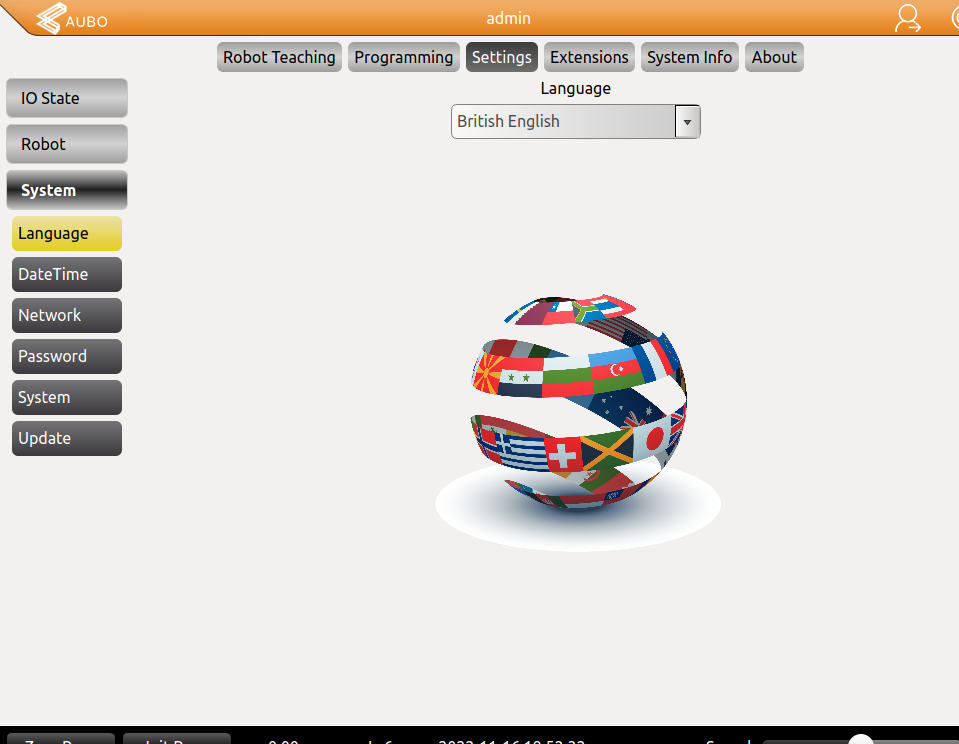
\includegraphics[width=\textwidth]{../../Images/settingsSystem.png}}
\end{center}
\item Select $'update'$ on the left
\begin{center}
  \makebox[\textwidth]{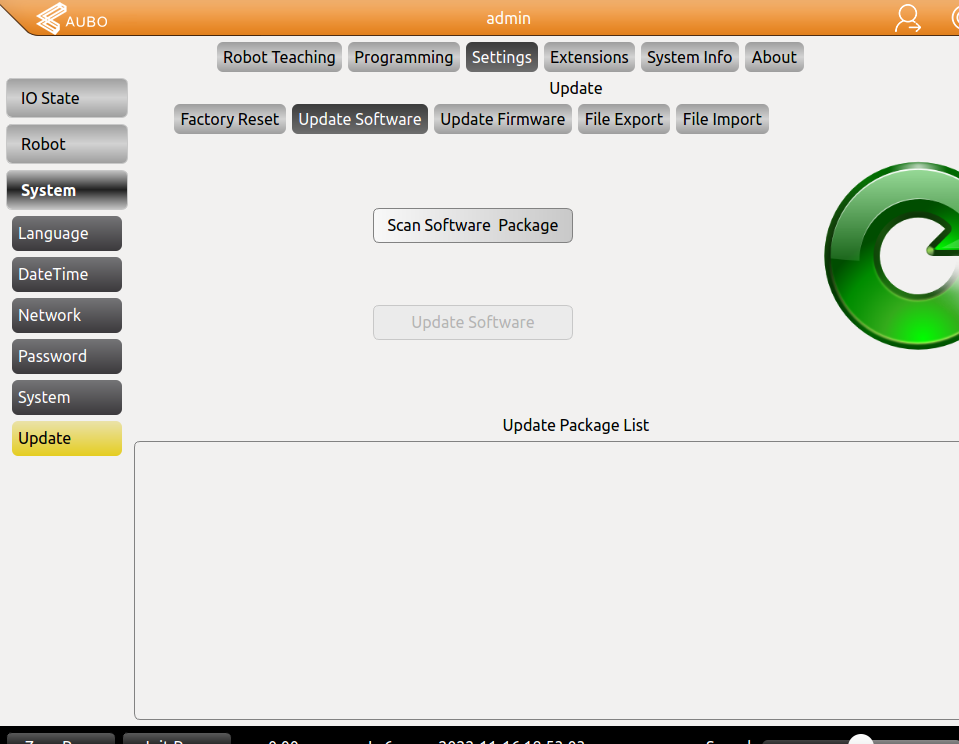
\includegraphics[width=\textwidth]{../../Images/update.png}}
\end{center}
\item select the $'File Export'$ tab. 
\begin{center}
  \makebox[\textwidth]{\includegraphics[width=\textwidth]{../../Images/FileExport.png}}
\end{center}
\item click $'Scan Device'$. Your usb should appear n the list. 
\item Select your USB and then press $'File Export'$
\end{itemize}

\subsubsection{Using a Backup}
\begin{itemize}
\item Acquire backupfile. Either from earlier or from a different machine you want to duplicate.
\item Move file to USB and plug USB into the robot.
\item Startup and login to the aubo robot. See \ref{subsec:Startup} and \ref{subsec:login}
\item Go to the $'Settings'$ tab.
\begin{center}
  \makebox[\textwidth]{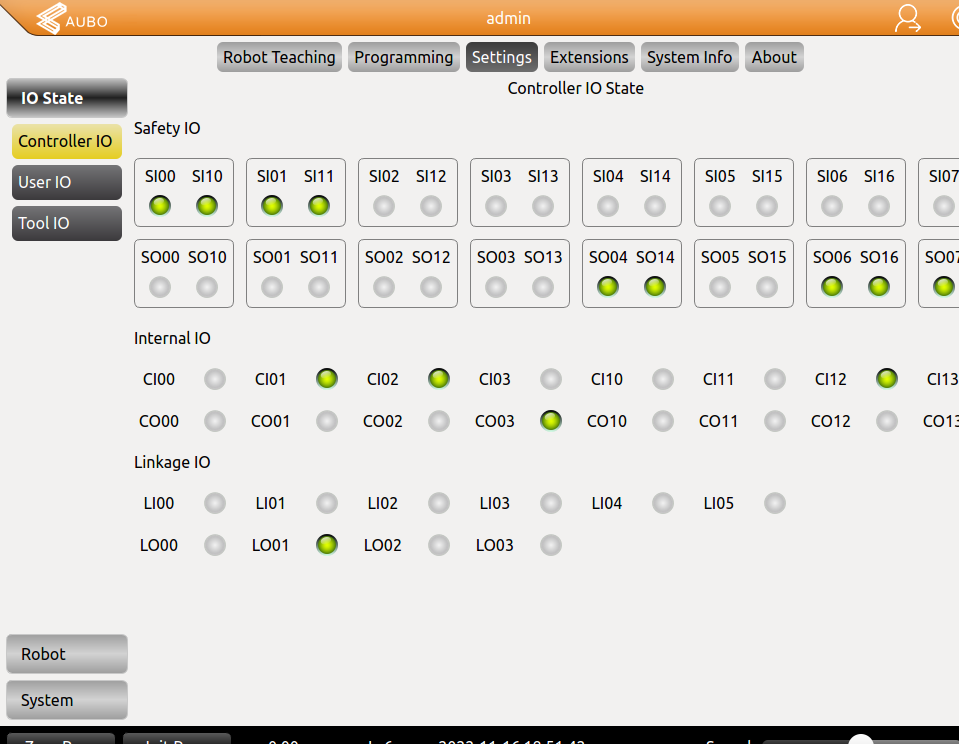
\includegraphics[width=\textwidth]{../../Images/settings.png}}
\end{center}
\item open the $'System'$ tab on the left
\begin{center}
  \makebox[\textwidth]{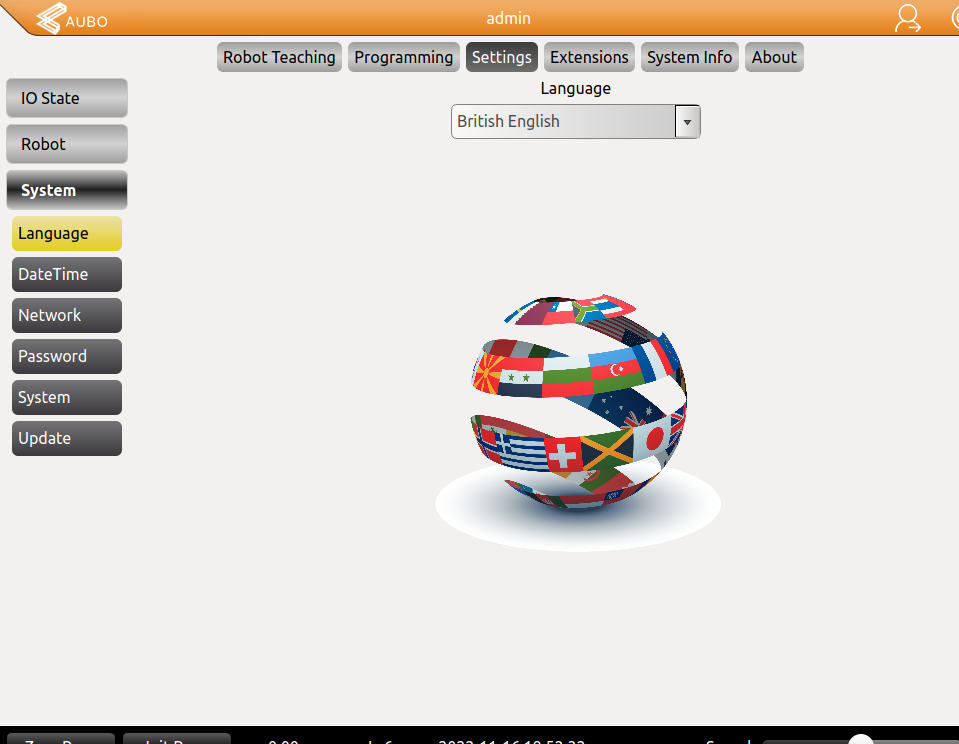
\includegraphics[width=\textwidth]{../../Images/settingsSystem.png}}
\end{center}
\item Select $'Update'$ on the left
\begin{center}
  \makebox[\textwidth]{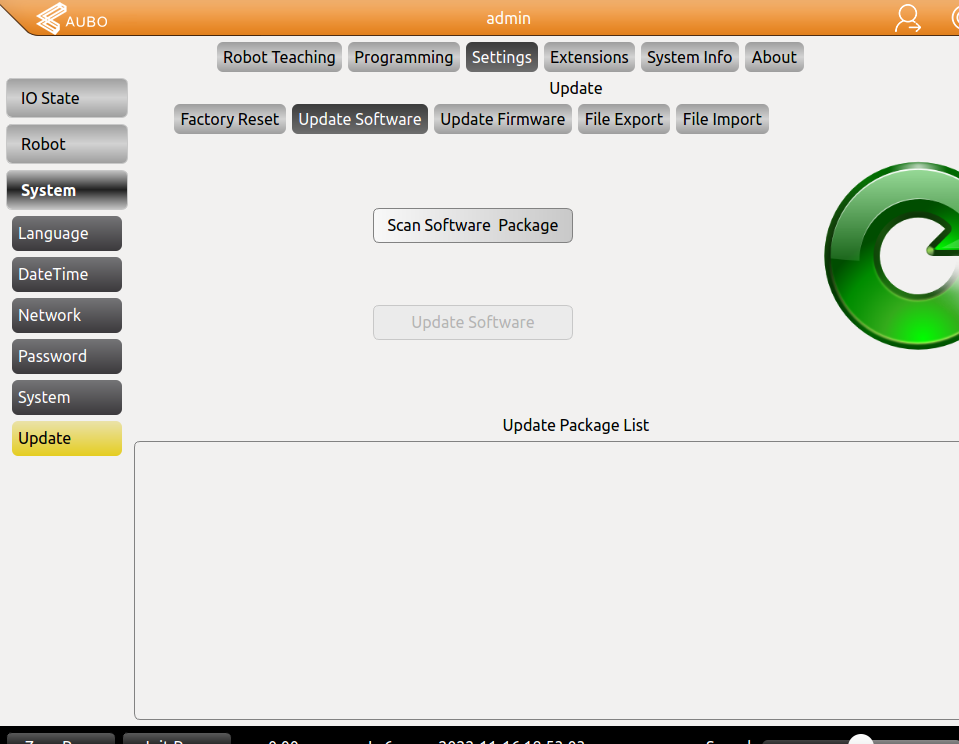
\includegraphics[width=\textwidth]{../../Images/update.png}}
\end{center}
\item Select the $'File Import'$ tab.
\begin{center}
  \makebox[\textwidth]{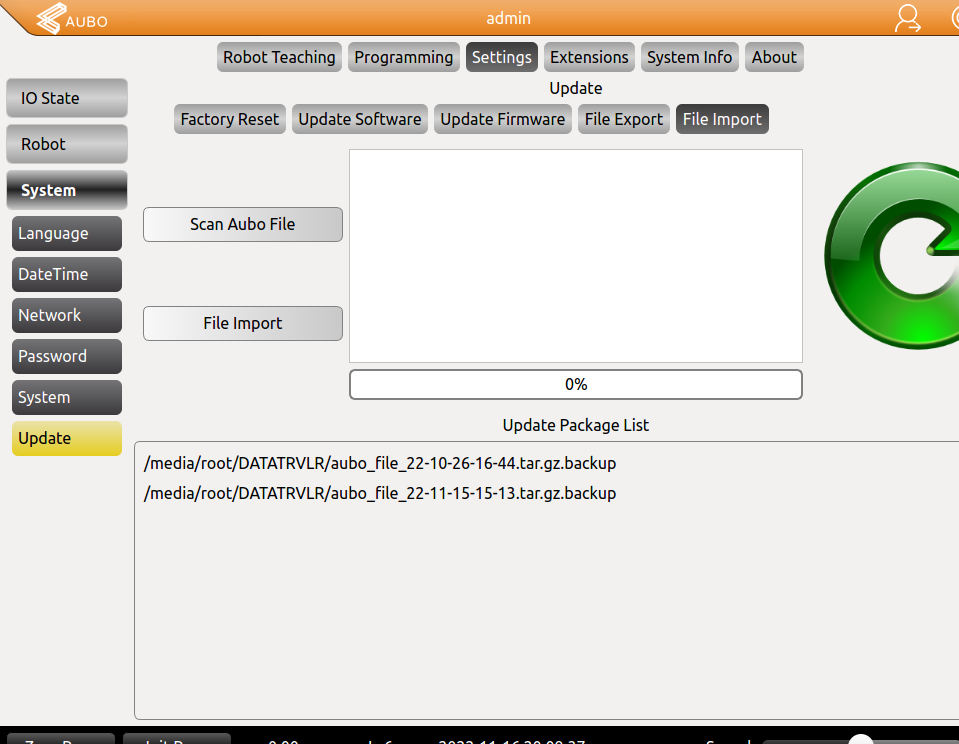
\includegraphics[width=\textwidth]{../../Images/FileImport.png}}
\end{center}
\item Click $Scan Aubo File$ and a list of the backup files on your USB should appear. 
\item Select the desired backup and press $'File Import'$
\item Wait a moment for the backup to install. 
\item Restart system. 
\item Check that your programs, variables, etc have been properly created.
\end{itemize}

\end{document}
